\documentclass[a4paper, titlepage]{article}
\title{Sobre cubrices y resultados de la extrapolación matricial.}
\author{Erik López de la Fuente}
\date{\today}

\usepackage[utf8]{inputenc}
\usepackage[spanish]{babel}
\usepackage{amsmath}
\usepackage{amsfonts}
\usepackage{enumerate}
\usepackage{graphicx}
\usepackage{float}

\counterwithin*{equation}{section}
\counterwithin*{equation}{subsection}
\counterwithin*{equation}{subsubsection}

\begin{document}

\maketitle
\tableofcontents
\newpage

\section{Definiciones.}

Sean $A \in M_{m\times n\times o} (\mathbb{K}), B \in M_{p\times q\times r} (\mathbb{K}), \Gamma \in M_{s\times t\times u} (\mathbb{K}), \Delta \in M_{v\times w\times x} (\mathbb{K})$. Definiremos:

\begin{itemize}
	\item Suma: $\Delta = A + B \Leftrightarrow \Delta_{ijk} = A_{ijk} + B_{ijk}$
	\item Producto cubricial: $\Delta = (A\cdot B\cdot \Gamma) \Leftrightarrow \Delta_{ijk} = \sum\limits_{l=1}^{z} A_{ilk} \cdot B_{ljk} \cdot \Gamma_{ijl}$, donde $z = n = p = u$, $v = \min \{m, s\}$, $w = \min \{q, t\}$ y $x = \min \{o, r\}$. (Piénsese en el máximo valor que puede alcanzar $l$ sin desbordar cada matriz).
	\item Producto por un escalar: $\Delta = a\cdot A \Leftrightarrow \Delta_{ijk} = a \cdot A_{ijk}$.
	\item Cubriz nula: $\vec{0}_{ijk} = 0$.
	\item Cubriz opuesta: $A + (-A) = \vec{0} \Leftrightarrow (-A)_{ijk} = -(A_{ijk})$.
\end{itemize}

% M_{nxnxn} es un espacio vectorial, pero el resto no porque el producto no es cerrado.

\section{Representaciones gráficas.}

\subsection{Bidimensional.}

Representamos a la cubriz como una serie de matrices separadas por barras verticales, donde cada matriz sería una ``rodaja'' ($k=1$, $k=2$...) de la cubriz.

\[ \left(
\begin{array}{c c c | c | c c c}
	\alpha_{111} & \cdots & \alpha_{1n1} &        & \alpha_{11o} & \cdots & \alpha_{1no} \\
	\vdots       &        & \vdots       & \cdots & \vdots       &        & \vdots       \\
	\alpha_{m11} & \cdots & \alpha_{mn1} &        & \alpha_{m1o} & \cdots & \alpha_{mno} \\
\end{array} \right)
\]

\subsection{Tridimensional superficial.}

\begin{figure}[H]
	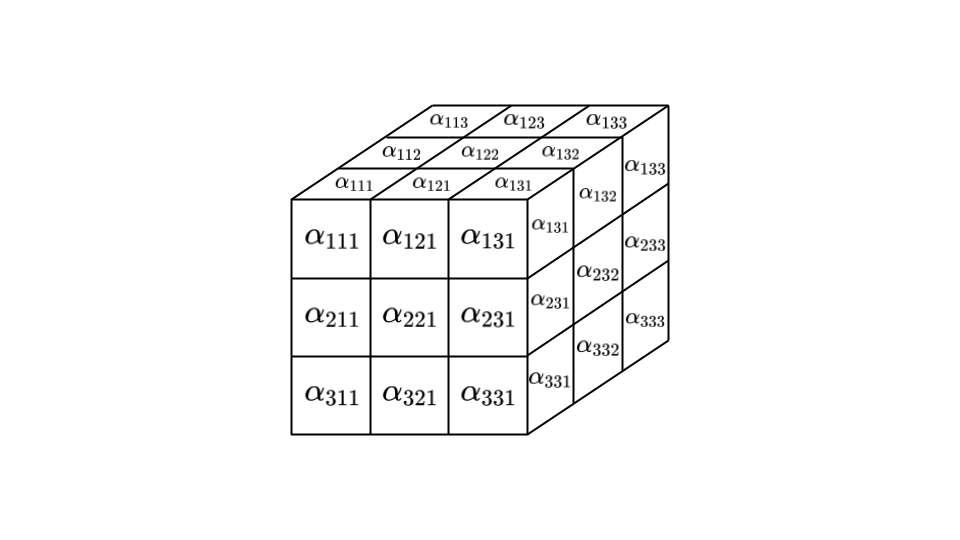
\includegraphics[width=\linewidth]{tridimensional_sup.png}
	\caption{Representación tridimensional superficial de una cubriz con elementos $\alpha_{ijk}$.}
\end{figure}

\subsection{Tridimensional completa.}

\begin{figure}[H]
	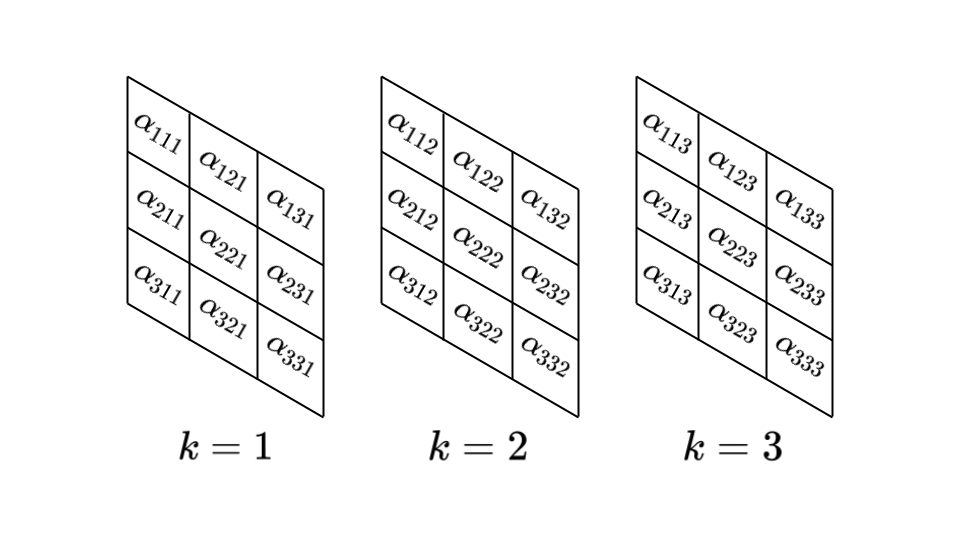
\includegraphics[width=\linewidth]{tridimensional_comp.png}
	\caption{Representación tridimensional completa de una cubriz con elementos $\alpha_{ijk}$.}
\end{figure}


\subsection{Producto.}

Bajo la definición ofrecida, el elemento $ijk$ de la cubriz $\Delta = (AB\Gamma)$ será igual al producto de la fila $i$ de $A$ por la columna $j$ de $B$ por la ''profundidad`` $k$ de $\Gamma$.

\begin{figure}[H]
	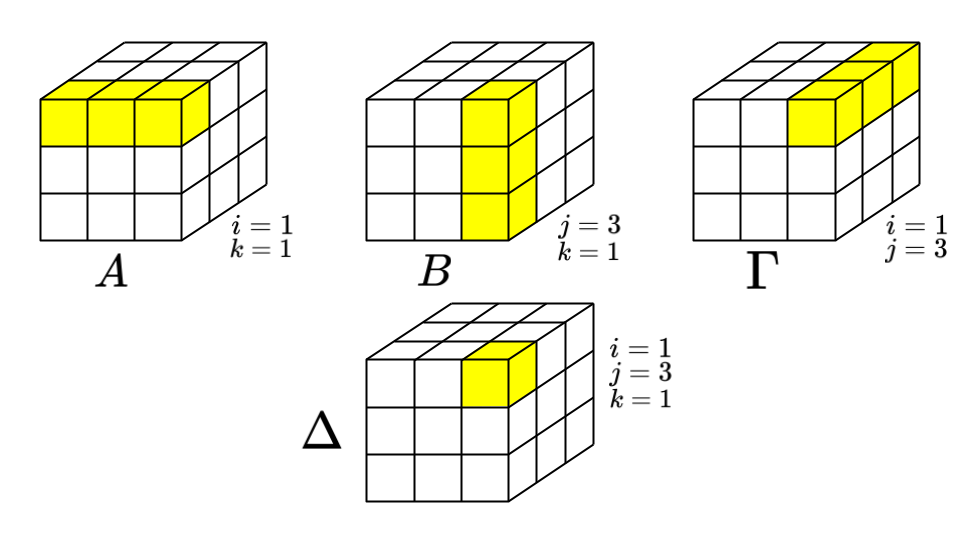
\includegraphics[width=\linewidth]{product.png}
	\caption{Representación tridimensional superficial del producto $\Delta = (AB\Gamma)$.}
\end{figure}

Esto explica las restricciones que marcan las dimensiones. En el proceso iterativo de la suma, es necesario que coincidan el número de columnas de $A$ ($n$), el número de filas de $B$ ($p$) y el número de ``profundidades'' de $\Gamma$ ($u$). Es esta cantidad común la que denominamos $z$ en la definición. Además, $\Delta$ no podrá tener más filas que $A$ ni que $\Gamma$ (de lo contrario, accederíamos a valores inexistentes), ni más columnas que $B$ o $\Gamma$, ni más ``profundidades'' que $A$ o $B$.

\section{En búsqueda de la identidad.}

La matriz identidad $I$ es aquélla tal que $AI = IA = A$. Es interesante buscar una noción similar en las cubrices.

\subsection{Caso particular: $2\times 2\times 2$.}

\subsubsection{Unicidad de I.}

Sean $A, I \in M_{2\times 2\times 2} (\mathbb{K})$. Partimos de tres asunciones:

\begin{itemize}
	\item Ningún elemento de $A$ es nulo.
	\item Los elementos de $I$ no dependen de $A$.
	\item La matriz identidad $I$ es única.
\end{itemize}

Con estas, desarrollemos la expresión del producto por definición:

\begin{equation}
A_{111} = I_{111} I_{111} A_{111} + I_{121} I_{211} A_{112}
\end{equation}

\begin{equation}
A_{112} = I_{112} I_{112} A_{111} + I_{122} I_{212} A_{112}
\end{equation}

\begin{equation}
A_{121} = I_{111} I_{121} A_{121} + I_{121} I_{221} A_{122}
\end{equation}

\begin{equation}
A_{122} = I_{112} I_{122} A_{121} + I_{122} I_{222} A_{122}
\end{equation}

\begin{equation}
A_{211} = I_{211} I_{111} A_{211} + I_{221} I_{211} A_{212}
\end{equation}

\begin{equation}
A_{212} = I_{212} I_{112} A_{211} + I_{222} I_{212} A_{212}
\end{equation}

\begin{equation}
A_{221} = I_{211} I_{121} A_{221} + I_{221} I_{221} A_{222}
\end{equation}

\begin{equation}
A_{222} = I_{212} I_{122} A_{221} + I_{222} I_{222} A_{222}
\end{equation}

En base a ese sistema derivamos lo siguiente:

\begin{enumerate}[(a)]
	\item Por $(1) \Rightarrow I_{111} = 1$.
	\item Por $(8) \Rightarrow I_{222} = 1$.
	\item Por $(3)$ y $(a) \Rightarrow I_{121} = 1$.
	\item Por $(3)$ y $(c) \Rightarrow I_{221} = 0$.
	\item Por $(6)$ y $(b) \Rightarrow I_{212} = 1$.
	\item Por $(2)$ y $(e) \Rightarrow I_{122} = 1$.
\end{enumerate}

Por $(8)$, o $I_{212}$ o $I_{122}$ deben ser $0$, pero por $(e)$ y $(f)$, $I_{212} = I_{122} = 1 \neq 0$. Surge la misma contradicción al probar con $IAI$ y $AII$.

Al menos una de nuestras suposiciones debe estar errada, y sería óptimo que fuese la tercera (sobre la unicidad de la identidad).

\subsubsection{La identidad como par.}

Decimos que $I, J$ es un \textit{par identidad} si cumple que $AIJ = A$ (exploraremos más adelante la influencia del orden de los factores).

Realizando el mismo desarrollo que antes, obtenemos el siguiente sistema:

\begin{equation}
A_{111} = A_{111} I_{111} J_{111} + A_{121} I_{211} J_{112}
\end{equation}

\begin{equation}
A_{112} = A_{112} I_{112} J_{111} + A_{122} I_{212} J_{112}
\end{equation}

\begin{equation}
A_{121} = A_{111} I_{121} J_{121} + A_{121} I_{221} J_{122}
\end{equation}

\begin{equation}
A_{122} = A_{112} I_{122} J_{121} + A_{122} I_{222} J_{122}
\end{equation}

\begin{equation}
A_{211} = A_{211} I_{111} J_{211} + A_{221} I_{211} J_{212}
\end{equation}

\begin{equation}
A_{212} = A_{212} I_{112} J_{211} + A_{222} I_{212} J_{212}
\end{equation}

\begin{equation}
A_{221} = A_{211} I_{121} J_{221} + A_{221} I_{221} J_{222}
\end{equation}

\begin{equation}
A_{222} = A_{212} I_{122} J_{221} + A_{222} I_{222} J_{222}
\end{equation}

De manera análoga, derivamos que:

\begin{enumerate}[(a)]
	\item Por $(1) \Rightarrow I_{111} \neq 0 \neq J_{111}$ y $I_{111} = J_{111}^{-1}$.
	\item Por $(8) \Rightarrow I_{222} \neq 0 \neq J_{222}$ y $I_{222} = J_{222}^{-1}$.
	\item Por $(2)$ y $(a) \Rightarrow I_{112} = J_{111}^{-1} = I_{111} \neq 0$.
	\item Por $(6)$ y $(c) \Rightarrow I_{112} = J_{211}^{-1} \neq 0 \Rightarrow J_{211} \neq 0$.
	\item Por $(5)$ y $(d) \Rightarrow J_{211} = I_{111}^{-1} = J_{111}$.
	\item Por $(7)$ y $(b) \Rightarrow I_{221} = J_{222}^{-1} \neq 0$.
	\item Por $(3)$, $(4)$ y $(f) \Rightarrow J_{122} = I_{221}^{-1} = I_{222}^{-1} = J_{222}^{-1}$.
	\item Por $(g)$ y $(b) \Rightarrow I_{222} = J_{222}^{-1} = I_{222}^{-1} \Rightarrow I_{222}^2 = 1 \Rightarrow I_{222} = 1 = J_{222}$.
\end{enumerate}

Recapitulando:

\begin{itemize}
	\item $I_{221} = J_{122} = I_{222} = J_{222} = 1$.
	\item $J_{211}^{-1} = I_{111} = J_{111}^{-1} = I_{112}$.
	\item El resto de términos:

	\begin{itemize}
		\item $I_{211} J_{112} = 0$.
		\item $I_{212} J_{112} = 0$.
		\item $I_{121} J_{121} = 0$.
		\item $I_{122} J_{121} = 0$.
		\item $I_{211} J_{212} = 0$.
		\item $I_{212} J_{212} = 0$.
		\item $I_{121} J_{221} = 0$.
		\item $I_{122} J_{221} = 0$.
	\end{itemize}
\end{itemize}

Dos cubrices cualquiera que cumplan estas condiciones serán consideradas un \textit{par identidad}, y cumplirán que $AIJ = A$. Es evidente entonces que si $\mathbb{K}$ es un cuerpo, existirán infinitos pares identidad, mientras que si es un anillo unitario conmutativo, solo existirán los que a continuación presentamos.

\subsection{Generalización.}

Por comodidad y estandarización, resulta inmediata la idea de establecer que todos los términos de la segunda condición sean iguales a $1$ y que todos aquéllos de la tercera lo sean a $0$. De esta manera, un par identidad estándar cumpliría que:

\begin{itemize}
	\item $1 = I_{221} = J_{122} = I_{222} = J_{222} = J_{211}^{-1} = I_{111} = J_{111}^{-1} = I_{112}$.
	\item $0 = I_{211} = J_{112} = I_{212} = J_{112} = I_{121} = J_{121} = I_{122} = J_{121} = I_{211} = J_{212} = I_{212} = J_{212} = I_{121} = J_{221} = I_{122} = J_{221}$.
\end{itemize}

Vemos que siempre se cumple que:

\begin{itemize}
	\item Si $j = 1 \rightarrow I_{1jk} = J_{ij1} = 1$ y $I_{2jk} = J_{ij2} = 0$.
	\item Si $j = 2 \rightarrow I_{1jk} = J_{ij1} = 0$ y $I_{2jk} = J_{ij2} = 1$.
\end{itemize}

El patrón se vuelve trivial si vemos qué ocurre con una cubriz $3 \times 3 \times 3$:

$$(AIJ)_{ijk} = A_{i1k} I_{1jk} J_{ij1} + A_{i2k} I_{2jk} J_{ij2} + A_{i3k} I_{3jk} J_{ij3}$$

\begin{itemize}
	\item Si $j = 1 \rightarrow I_{1jk} = J_{ij1} = 1$ y $I_{2jk} = J_{ij2} = 0$ y $I_{3jk} = J_{ij3} = 0$.
	\item Si $j = 2 \rightarrow I_{1jk} = J_{ij1} = 0$ y $I_{2jk} = J_{ij2} = 1$ y $I_{3jk} = J_{ij3} = 0$.
	\item Si $j = 3 \rightarrow I_{1jk} = J_{ij1} = 0$ y $I_{2jk} = J_{ij2} = 0$ y $I_{3jk} = J_{ij3} = 1$.
\end{itemize}

Es decir, para que $(AIJ)_{ijk} = A_{ijk}$, debe cumplirse que $I_{ljk} = J_{ijl} = \delta_{jl}$, donde

\begin{equation}
	\delta_{jl} =
	\begin{cases}
		1 & \text{si } j = l \\
		0 & \text{si } j \neq l
	\end{cases}
\end{equation}

Pero para $I$, que $j = l$ equivale a que $i = j$. Es así que llegamos a la siguiente expresión independiente:

$$I_{ijk} = \delta_{ij}$$

\subsection{Las tres Kronecker}

Es sencillo hacer un desarrollo similar tanto para $I_2AJ_2$ como para $I_3J_3A$ (téngase en mente que el par identidad no es conmutativo), del cual obtendremos que:

\begin{itemize}
	\item $AI_1J_1 = A \Leftrightarrow I_1 = \delta_{ij}$ y $J_1 = \delta_{jk}$.
	\item $I_2AJ_2 = A \Leftrightarrow I_2 = \delta_{ij}$ y $J_2 = \delta_{ik}$.
	\item $I_3J_3A = A \Leftrightarrow I_3 = \delta_{jk}$ y $J_3 = \delta_{ik}$.
\end{itemize}

Con esto concluímos que existen tres pares identidad estándar fundamentados sobre las tres Kronecker. No es inmediatamente obvio qué patrón se puede esclarecer de este resultado. Una posibilidad es la siguiente:

\begin{itemize}
	\item Si $I$ es adyacente a $A$, $I = \delta_{ij}$. Si no, $I = \delta_{jk}$.
	\item Si $J$ es adyacente a $A$, $J = \delta_{ik}$. Si no, $J = \delta_{jk}$.
\end{itemize}

Sea como fuere, es intrigante observar los patrones dibujados por cada Kronecker. Tomemos sus representaciones tridimensionales completas.


\begin{figure}[H]
	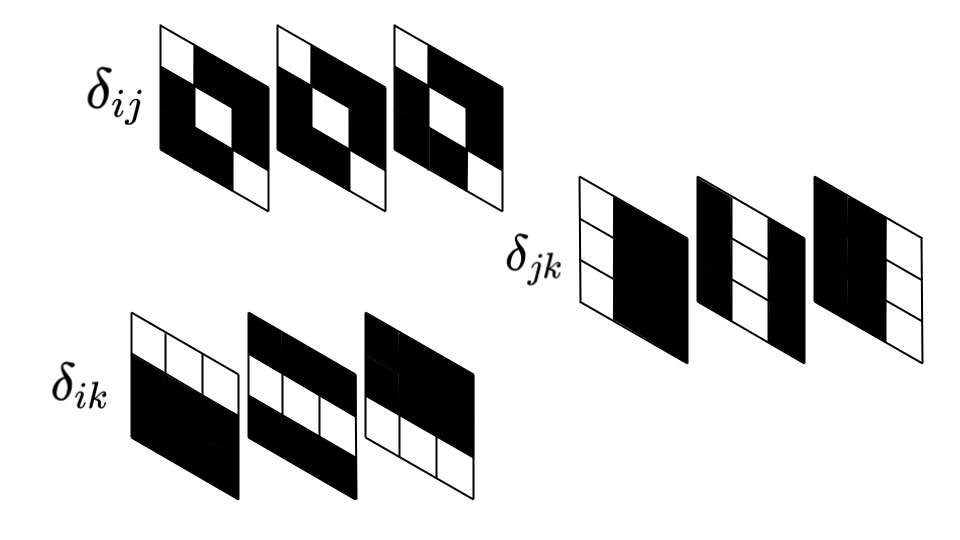
\includegraphics[width=\linewidth]{kroneckers.png}
	\caption{Representación tridimensional completa de $\delta_{ij}$, $\delta{jk}$ y $\delta{ik}$ (celdas iguales a $1$ en blanco e iguales a $0$ en negro).}
\end{figure}

\section{Conclusión}

Tras este análisis descubrimos que las cubrices conforman un conjunto verdaderamente interesante a la par que misterioso. Este desarrollo teórico no aspira a encontrar grandes usos para estos objetos matemáticos, sino más bien explorar una posible extrapolación al concepto de matriz.

\end{document}
